%\section{Methods}
\label{sec:methods}

Our data structure for colored de Bruijn graphs is based on the succinct representation of individual de Bruijn graphs introduced by \cite{BOSS12}---which we refer to as the BOSS representation from the authors' initials---so we start by describing that representation.  We note that BOSS is itself a generalization of FM-indexes~\citep{FM05} obtained by extending the Burrows-Wheeler transform (BWT) from strings to the multisets of edge-labels of de Bruijn graphs.  We then give a general explanation of how we add colors, and finally give details of our implementation.

\subsection{BOSS Representation}
\label{subsec:boss}

Consider the de Bruijn graph \(G = (V, E)\) for a set of $k$-mers, with each $k$-mer \(a_0 \cdots a_{k - 1}\) representing a directed edge from the node labelled \(a_0 \cdots a_{k - 2}\) to the node labelled \(a_1 \cdots a_{k - 1}\), with the edge itself labelled \(a_{k - 1}\).  Define the nodes' co-lexicographic order to be the lexicographic order of their reversed labels.  Let $F$ be the list of $G$'s edges sorted co-lexicographically by their ending nodes, with ties broken co-lexicographically by their starting nodes (or, equivalently, by their $k$-mers' first characters).  Let $L$ be the list of $G$'s edges sorted co-lexicographically by their starting nodes, with ties broken co-lexicographically by their ending nodes (or, equivalently, by their own labels).  If two edges $e$ and $e'$ have the same label, then they have the same relative order in both lists; otherwise, their relative order in $F$ is the same as their labels' lexicographic order.  Defining the edge-BWT (EBWT) of $G$ to be the sequence of edge labels sorted according to the edges' order in $L$, so \(\elabel (L [h]) = \EBWT (G) [h]\) for all $h$, this means that if $e$ is in position $p$ in $L$, then in $F$ it is in position
\begin{equation*}
|\{d\,:\,d \in E,\ \elabel (d) \prec \elabel (e)\}| + \EBWT (G).\rank_{\elabel (e)} (p) - 1\,,
\end{equation*}
where \(\EBWT (G).\rank_{\elabel (e)} (p)\) is the number of times $\elabel (e)$ appears in \(\EBWT (G) [1,p]\).  It follows that if we have, first, an array storing \(|\{d\,:\,d \in E,\ \elabel (d) \prec c\}|\) for each character $c$ and, second, a fast rank data structure on \(\EBWT (G)\) then, given an edge's position in $L$, we can quickly compute its position in $F$.

Let $B_F$ be the bitvector with a 1 marking the position in $F$ of the last incoming edge of each node, and let $B_L$ be the bitvector with a 1 marking the position in $L$ of the last outgoing edge of each node.  Given a character $c$ and the co-lexicographic rank of a node $v$, we can use $B_L$ to find the interval in $L$ containing $v$'s outgoing edges, then we can search in \(\EBWT (G)\) to find the position of the one $e$ labelled $c$.  We can then find $e$'s position in $F$, as described above.  Finally, we can use $B_F$ to find the co-lexicographic rank of $e$'s ending node.  With the appropriate implementations of the data structures, we can store $G$ in \((1 + o (1)) |E| (\lg \sigma + 2)\) bits, where $\sigma$ is the size of the alphabet (i.e., 4 for DNA), such that when given a character $c$ and the co-lexicographic rank of a node $v$, in $\Oh{\log \log \sigma}$ time we can find the node reached from $v$ by following the directed edge labelled $c$, if such an edge exists.

If we know the range \(L [i..j]\) of $k$-mers whose starting nodes end with a pattern $P$ of length less than \((k - 1)\), then we can compute the range \(F [i'..j']\) of $k$-mers whose ending nodes end with \(P c\), for any character $c$, since
\begin{eqnarray*}
    i' & = & |\{d\,:\,d \in E,\ \elabel (d) \prec c\}| + \EBWT (G).\rank_c (i - 1)\\ 
    j' & = & |\{d\,:\,d \in E,\ \elabel (d) \prec c\}| + \EBWT (G).\rank_c (j) - 1\,.
\end{eqnarray*}
It follows that, given a node $v$'s label, we can find the interval in $L$ containing $v$'s outgoing edges in $\Oh{k \log \log \sigma}$ time, provided there is a directed path to $v$ (not necessarily simple) of length at least \(k - 1\).  In general there is no way, however, to use \(\EBWT (G)\), $B_F$ and $B_L$ alone to recover the labels of nodes with no incoming edges.

To prevent information being lost and to be able to support searching for any node given its label, Bowe et al.\ add extra nodes and edges to the graph, such that there is a directed path of length at least \(k - 1\) to each original node.  Each new node's label is a \((k - 1)\)-mer that is prefixed by one or more copies of a special symbol $\$$ not in the alphabet and lexicographically strictly less than all others.  Notice that, when new nodes are added, the node labelled $\$^{k - 1}$ is always first in co-lexicographic order and has no incoming edges.  Bowe et al.\ also attach an extra outgoing edge labelled $\$$, that leads nowhere, to each node with no original outgoing edge.  The edge-BWT and bitvectors for this augmented graph are, together, the BOSS representation of $G$.

\subsection{Adding Color}
\label{subsec:color}

We cannot represent the colored de Bruijn graph for a multiset \(\mathcal{G} = \{G_1, \ldots, G_t\}\) of individual de Bruijn graphs satisfactorily by simply representing each individual graph separately, for two reasons: first, the memory requirements would quickly become impractical and, second, we should be able to answer efficiently queries such as ``which individual graphs contain this edge?''  Therefore, we set $G$ to be the union of the individual graphs and build the BOSS representation only for $G$.  As long as most of the $k$-mers are common to most of the individual graphs, the memory needed to store $G$ is comparable to that need to store an individual graph.

To indicate which edges of $G$ are in which individual graphs, we build and store a two-dimensional binary array $C$ in which \(C [i, j]\) indicates whether the $i$th edge in $G$ is present in the $j$th individual de Bruijn graph (i.e., whether that edge has the $j$th color). 
(Recall from the description above of BOSS that we consider the edges in $G$ to be sorted lexicographically by the reversed labels of their starting nodes, with ties broken lexicographically by their own single-character labels.) 
If the individual graphs are sufficiently similar, then we can compress $C$ effectively and store it in such a way that we can still access its individual bits quickly and support fast rank and select queries on the rows.  (A $\select$ query on the $i$th row takes an argument $r$ and returns the index $j$ of the $r$th individual graph that contains the $i$th edge in $G$.)  In the next subsection we give details of some relatively simple compression strategies that support fast access, rank and select.  With these data structures, we can navigate efficiently in any of the individual graphs and switch between them.  For example, we can efficiently check whether an edge has a particular color (with an access), count the number of colors it has (with a $\rank$ query) or list them (with repeated $\select$ queries).  We have not yet considered more sophisticated compression schemes that could still offer fast queries while taking advantage of, e.g., correlations among the variations or grouping of the individual graphs by subpopulation.

Figure~\ref{fig:purple} shows an example of how we represent a colored de Bruijn graph consisting of two individual de Bruijn graphs.  Suppose we are at node {\tt ACG} in the graph, which is the co-lexicographically eighth node.  Since the eighth 1 in $B_L$ is \(B_L [10]\) and it is preceded by two 0s, we see that {\tt ACG}'s outgoing edges' labels are in \(\EBWT [8..10]\), so they are {\tt A}, {\tt C} and {\tt T}.  Suppose we want to follow the outgoing edge $e$ labelled {\tt C}.  We see from \(C [9, 0..1]\) (i.e., the tenth column in $C^\mathrm{T}$) that $e$ appears in the second individual graph but not the first one (i.e., it is blue but not red).    There are four edges labelled {\tt A} in the graph and three {\tt C}s in \(\EBWT (G) [0..9]\), so $e$ is \(F [6]\).  (Since edges labelled {\tt \$} have only one end, they are not included in $L$ or $F$.)  From counting the 1s in \(B_F [0..6]\), we see that $e$ arrives at the fifth node in co-lexicographic order that has incoming edges.  Since the first node, {\tt \$\$\$}, has no incoming edges, that means $e$ arrives at the sixth node in co-lexicographic order, {\tt CGC}.

\begin{figure*}
\begin{tabular}{c@{\hspace{0.03\textwidth}}c@{\hspace{0.03\textwidth}}c}
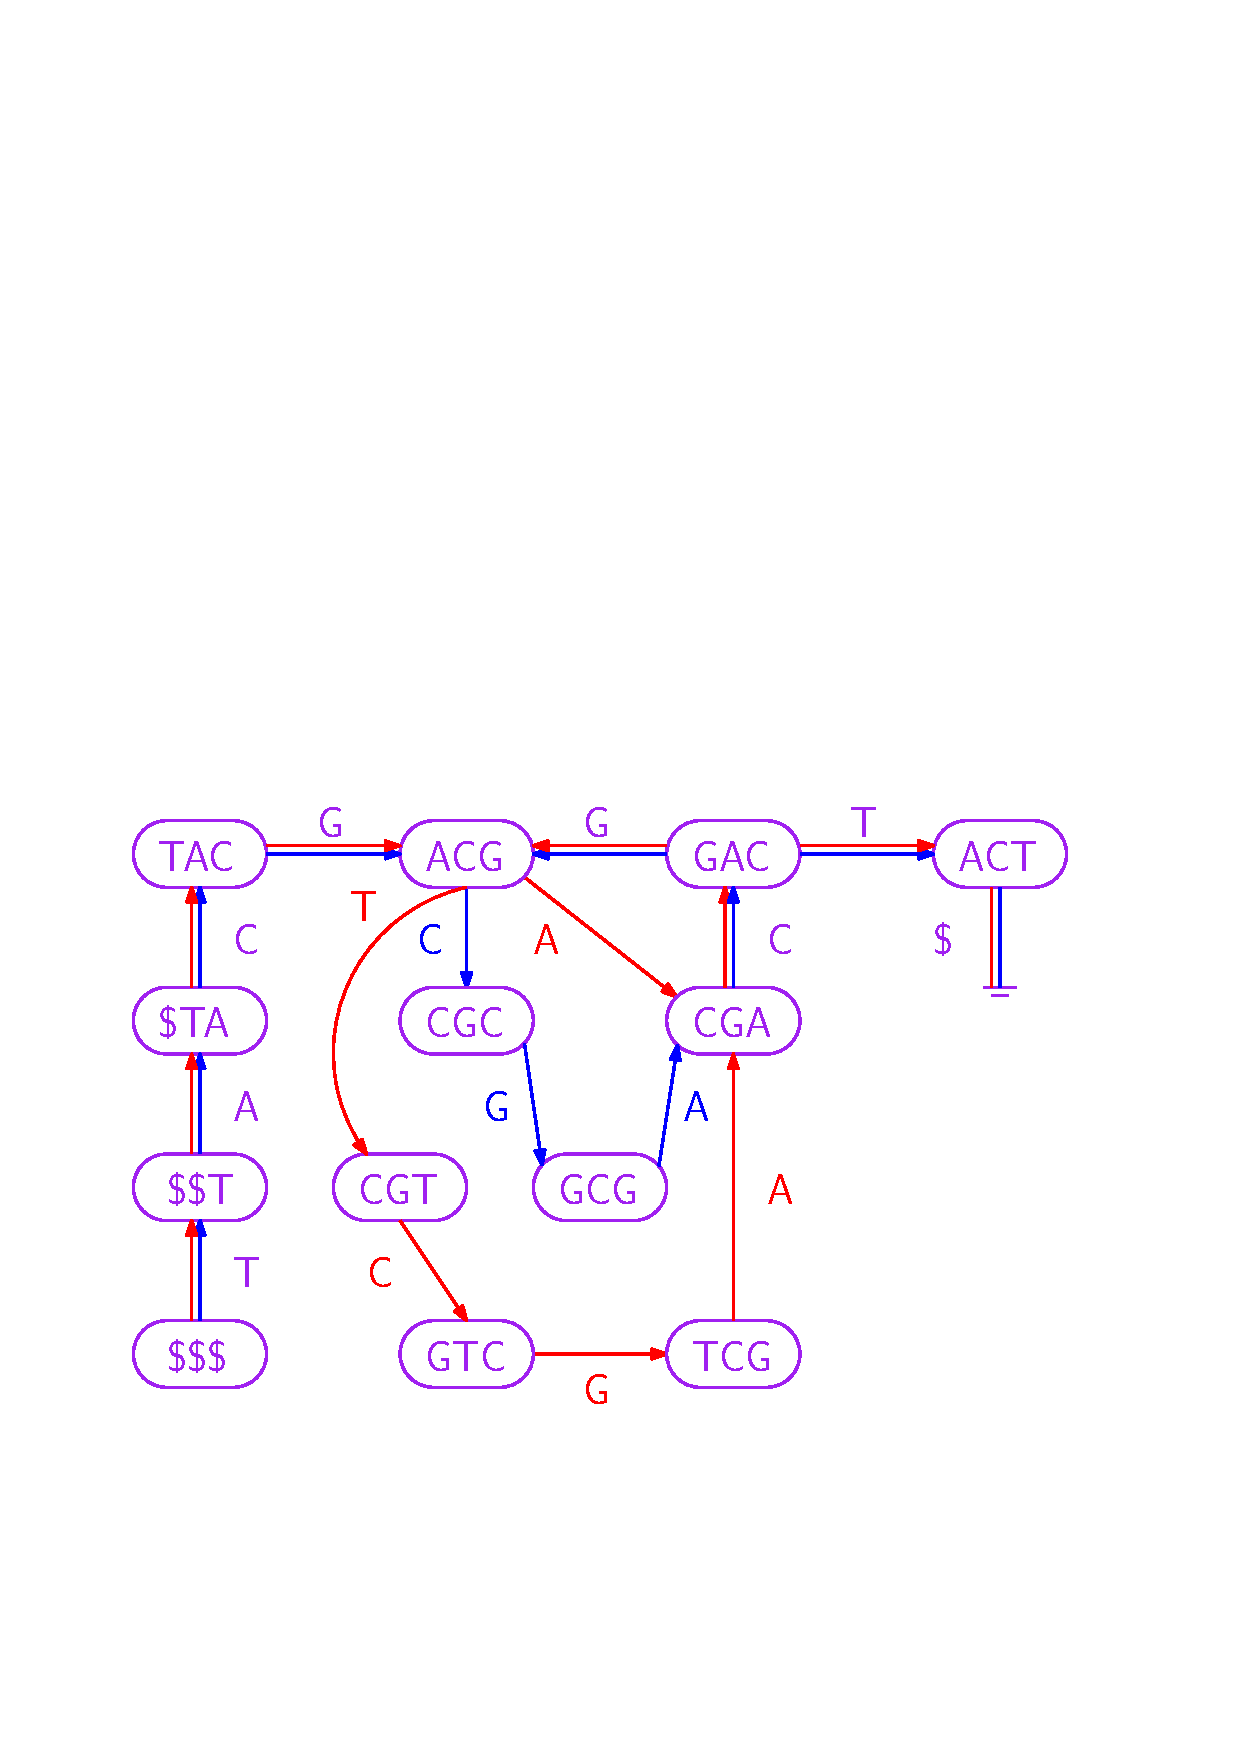
\includegraphics[width=.31\textwidth]{purplegraph} &
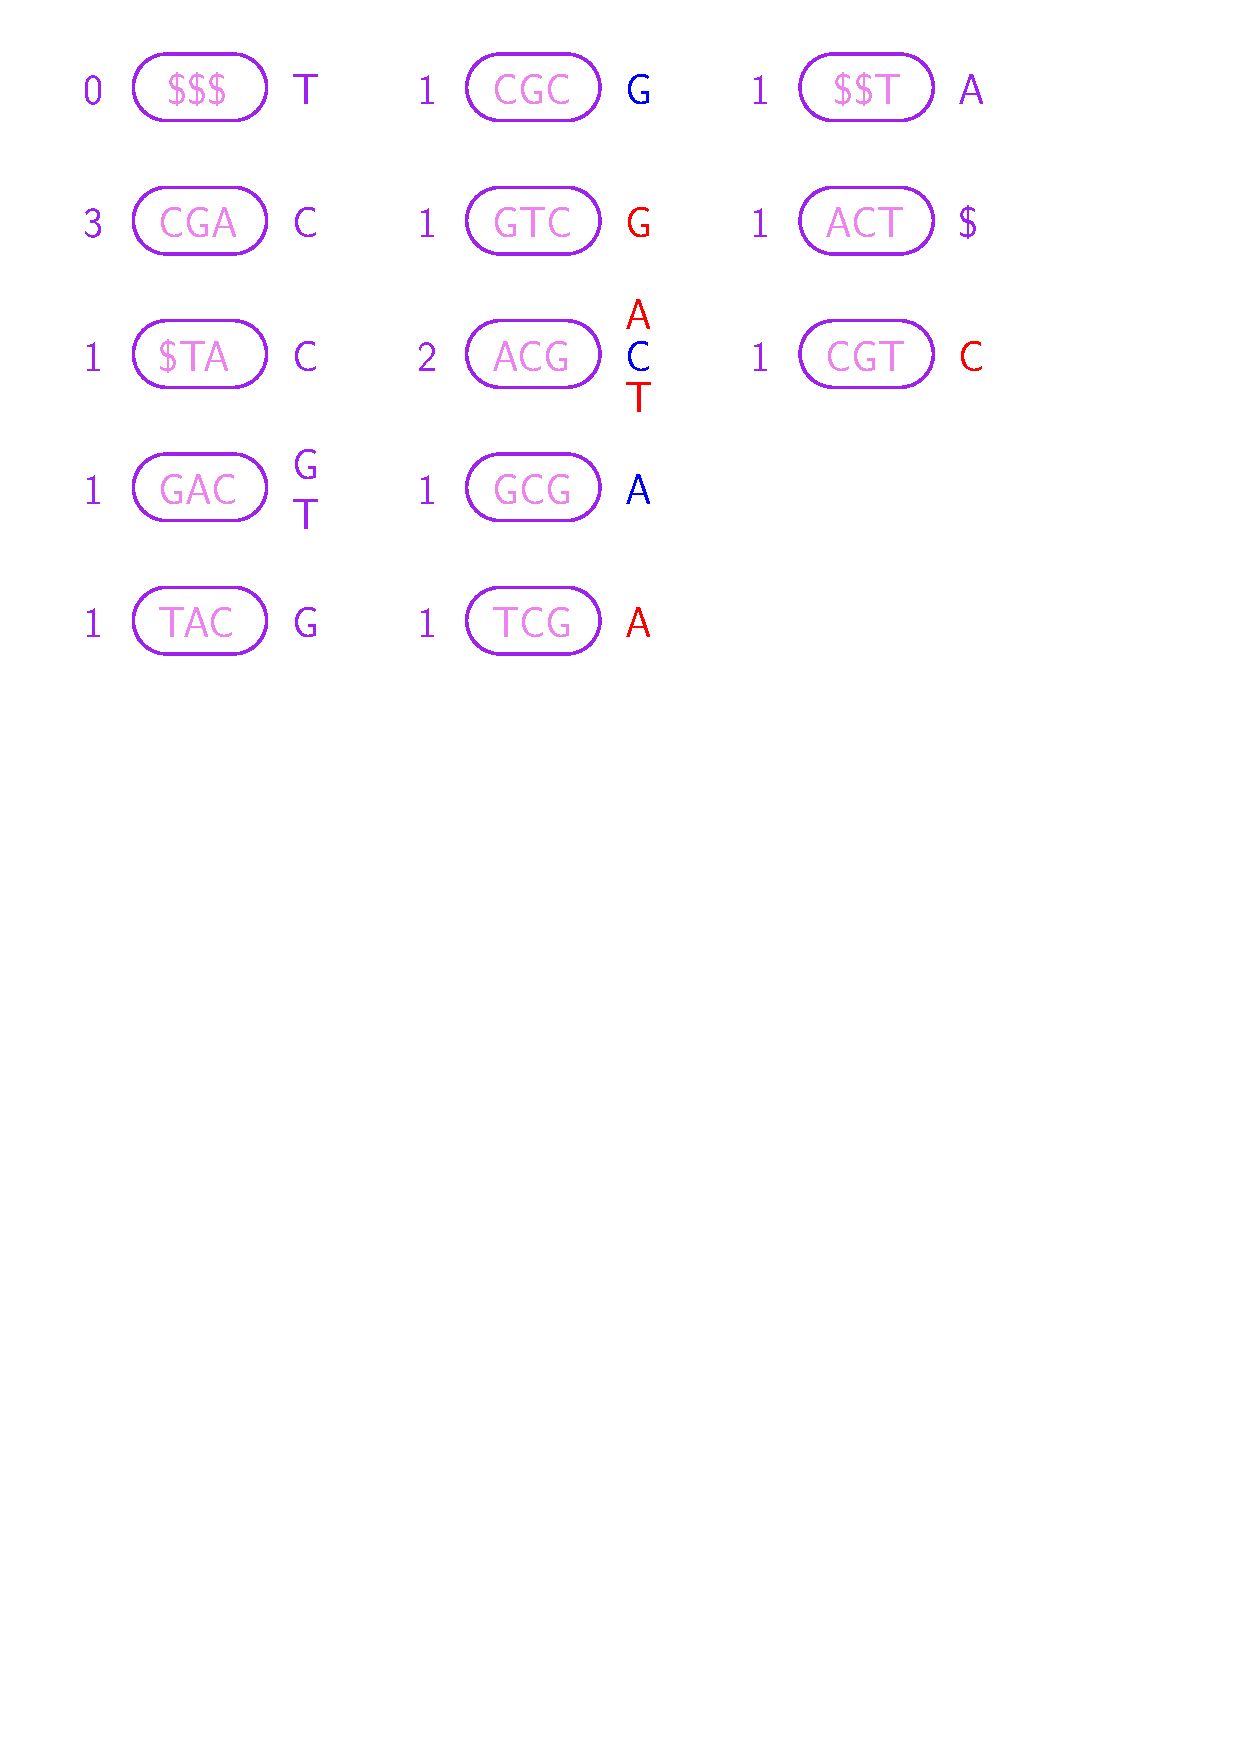
\includegraphics[width=.31\textwidth]{newpurplemapping} &
\raisebox{11ex}{$\begin{array}{rr}
   \EBWT (G) = & \mathtt{TCCGTGGGACTAAA\$C}\\[1ex]
         B_F = & \mathtt{ 001111110111111}\\
         B_L = & \mathtt{1110111100111111}\\[1ex]
C^\mathrm{T} = & \mathtt{0000001001010000}\\
               & \mathtt{0000000110101001}
\end{array}$}
\end{tabular}
\caption{{\bf Left:} A colored de Bruijn graph consisting of two individual graphs, whose edges are shown in red and blue.  (We can consider all nodes to be present in both graphs, so they are shown in purple.)  {\bf Center:} The nodes sorted into co-lexicographic order, with each node's number of incoming edges shown on its left and the labels of its outgoing edges shown on its right.  The edge labels are shown in red or blue if the edges occur only in the respective graph, or purple if they occur in both.  {\bf Right:} Our representation of the colored de Bruijn graph: the edge-BWT and bitvectors for the BOSS representation for the union of the individual graphs, and the binary array $C$ (shown transposed) whose bits indicate which edges are present in which individual graphs.}
\label{fig:purple}
\end{figure*}

\subsection{Implementation}
\label{subsec:implementation}

We now give some details of how our data structure is implemented and constructed in practice.

\subsubsection{Data Structure}

The arsenal of component tools available to succinct data structures designers has grown considerably in recent years~\citep{Navarro16}, with many methods now implemented in libraries. We chose to make heavy use of the succinct data structures library (SDSL)\footnote{\url{https://github.com/simongog/sdsl-lite}} 
in our implementation.

\(\EBWT (G)\), the sequence of edge labels, is encoded in a wavelet tree, which allows us to perform fast rank queries, essential to all our graph navigations. The bitvectors of the wavelet tree  and the $B$ bitvector are stored in the Raman-Raman-Rao (RRR) encoding~\citep{RRR07}.
%[SJP: RRR will be significantly slower than a plain encoding, and I'm not sure it will reduce the size of the WT very much - this is something we need to test. We might even want to use something other than a WT].
The rows of the color matrix, $C$, are concatenated (i.e. $C$ is stored in row-major order) and this single long bit string is then compressed.  It is either stored with RRR encoding,  or alternately Elias-Fano encoding~\citep{elias1974efficient,fano1971number,bitvector} which supports online construction.  Online construction is important for datasets where $C$ is too large to fit in memory in uncompressed form, such as our metagenomic sample dataset.  These encodings reduce the size of $C$ considerably because we expect rows to be very sparse
%(i.e. most $k$-mers are contained in most samples),
and both encodings exploit this sparseness. 
%[SJP: we really should be using the access-optimised encoding that Travis and I suggested --- RRR is overkill and likely slower].

\subsubsection{Construction}

\chapter{Space-efficient CSA construction}\label{chapter:construction}

In this chapter, we investigate the direct construction of compressed suffix arrays, extending the results in Paper~II. We are mostly interested in algorithms whose space usage is dominated by the CSA itself, making it possible to build indexes for texts that are larger than memory size.

The standard way of constructing compressed suffix arrays is to build a suffix array first, and then compress it. There are many existing algorithms \cite{Puglisi2007}, with the best of them working in $O(n)$ time and requiring $2n$ bits of working space in addition to the text and the suffix array \cite{Nong2009}. Yet as a compressed suffix array usually requires less than $n$ bytes of memory \cite{Ferragina2009a}, and can take less than $n$ \emph{bits} with highly repetitive texts (see Section~\ref{sect:rlcsa experiments}), this approach limits the use of CSAs to much smaller texts than could be handled in the available memory.

Many of the suffix array construction algorithms can be adapted to construct the Burrows-Wheeler transform directly. This often replaces the $4n$ to $8n$-byte suffix array with a $n$-byte BWT, reducing memory usage considerably. Yet even the best algorithms \cite{Kaerkkaeinen2007,Okanohara2009} require the text or the BWT --- or both --- in memory, limiting the size of the texts that can be indexed. External memory algorithms for constructing the suffix array \cite{Dementiev2008a} and the Burrows-Wheeler transform \cite{Ferragina2012} exist, but they tend to be slow in practice. In principle, dynamic self-indexes (see Section~\ref{sect:dynamic indexes}) could be used for space-efficient CSA construction, but the implementations seen so far are both slower and require more memory than the alternatives.

Direct algorithms for compressed suffix array construction \cite{Hon2007,Na2007,Hon2009} are the best solution so far. We are especially interested in the algorithm of Hon \etal{Hon2007} that works in $O(n \log n)$ time and requires $\abs{\CSA} + O(n)$ bits of memory. The algorithm essentially uses a static index to simulate CSA construction by a dynamic index, inserting many suffixes in a single update. We describe two practical variants of this algorithm: one that is more space-efficient and another one that can be faster than the original. As the basic building block, we describe an algorithm for merging compressed suffix arrays.

A similar idea has been recently used for constructing the Burrows-Wheeler transform for a large collection of short texts in external memory \cite{Bauer2011}. Instead of inserting large blocks of text at once, the algorithm extends each text by a single character in each step. This way, the algorithm remains simple and has to maintain only a small amount of state information, making it fast and space-efficient in practice. On the other hand, if the texts are longer than a few hundred characters, the algorithm requires too many passes over the data to be useful.


\section{Merging Burrows-Wheeler transforms}\label{sect:merging}

\paragraph{Algorithm of Hon et al.}

The construction algorithm of Hon \etal{Hon2007} can be interpreted as updating the Burrows-Wheeler transform of a text. Assume that we have already constructed $\BWT$ for some text $T$, and we want to update it for $ST$, where $S$ is a sequence of length $l$. We call the suffixes of $ST$ starting in $S$ the \emph{long suffixes} of $ST$, and the rest of the suffixes \emph{short suffixes}.

\begin{definition}
Let $T$ and $T'$ be two texts. The \emph{rank array} $\RA[1,\abs{T'}]$ of text $T'$ relative to text $T$ is an array such that $\RA[i] = \mrank(T, T'[i,\abs{T'}])$. The rank array of a set of suffixes of text $T'$ relative to text $T$ is the corresponding subsequence of array $\RA$.
\end{definition}

The definition also generalizes for collections of texts.

Updating the BWT starts with computing the rank array of long suffixes of text $ST$ relative to text $T$. Backward searching can be used to compute the rank array in a similar way as in the update rule for dynamic compressed suffix arrays (see Section~\ref{sect:dynamic indexes}). A detailed algorithm can be found in Figure~\ref{fig:rank array}.

\begin{figure}
\begin{tabbing}
mm\=mm\=mm\= \kill
\> \textbf{function} $\operatorname{computeRanks}(\mrank(T,T), S, l)$ \\
\> \> $pos \leftarrow \mrank(T, T)$ \\
\> \> \textbf{for} $i \leftarrow l$ \textbf{to} $1$ \\
\> \> \> $pos \leftarrow C[S[i]] + \mrank_{S[i]}(\BWT, pos) + 1$ \\
\> \> \> $\RA[i] \leftarrow pos$ \\
\> \> \textbf{return} $\RA$
\end{tabbing}

\caption{Computing the rank array of long suffixes of text $ST$ relative to text $T$ by backward searching the Burrows-Wheeler transform of $T$.}\label{fig:rank array}
\end{figure}

In addition to determining the lexicographic ranks of long suffixes among short suffixes, we must also determine their ranks among themselves. Conceptually this is done by sorting the long suffixes by their first $l$ characters, breaking ties by using the suffix array of $T$. With both ranks, we can determine the lexicographic ranks of long suffixes among all suffixes.

\begin{lemma}[Fact 1 in \cite{Hon2007}]
The lexicographic rank of a long suffix $S'$ among all suffixes of $ST$ is the sum of its lexicographic ranks among long suffixes and among short suffixes.
\end{lemma}

At this point, we have the lexicographic ranks among long suffixes in suffix array order, and the ranks among short suffixes in text order. By sorting the rank array in increasing order, we get both ranks in suffix array order. This follows from the fact that $S_{1} < S_{2}$ implies $\mrank(T, S_{1}) \le \mrank(T, S_{2})$. Hence the lexicographic ranks of long suffixes among short suffixes must form a non-decreasing sequence, when put into suffix array order. The entire merging algorithm is as follows.

\begin{enumerate}

\item Determine the rank array $\RA$ by the algorithm in Figure~\ref{fig:rank array}. Sort it to get array $\RA'$, and update this array by rule $\RA'[i] \leftarrow \RA'[i] + i$ to get the lexicographic ranks of long suffixes among all suffixes.

\item Sort the long suffixes, and form $\BWT_{S}$ as the subsequence of $\BWT_{ST}$ corresponding to the long suffixes.

\item Update $\BWT_{T}[\mrank(T, T)] \leftarrow S[l]$, and then merge $\BWT_{S}$ and $\BWT_{T}$ to get $\BWT_{ST}$. The merging is done by inserting characters from $\BWT_{S}$ to positions marked in $\RA'$, filling the rest of the positions with characters from $\BWT_{T}$.

\end{enumerate}

\begin{lemma}[Lemma 10 in \cite{Hon2007}]
The above algorithm updates $\BWT_{T}$ to $\BWT_{ST}$ in $O(l \log n + n)$ time, requiring $4l \log n + n + o(n)$ bits of space in addition to $\BWT_{S}$ and $\BWT_{T}$.
\end{lemma}

\paragraph{Merging compressed suffix arrays.}

A simplified version of the above algorithm can be used to merge two compressed suffix arrays. Assume that we have compressed suffix arrays for two texts $T$ and $T'$, and we want to merge them to get a compressed suffix array for the collection $\mathcal{C} = \set{T, T'}$. We select $\CSA_{T}$ as the basic index, and update it to get $\CSA_{\mathcal{C}}$.

In step 1, we get the rank array by searching $\CSA_{T}$ for text $T'$. However, as we are inserting entire texts instead of extending existing texts, we start with $\RA[\abs{T'}] = 1$, as the end marker of $T'$ will come immediately after the end marker of $T$ in lexicographic order. Step 2 is not needed, as we already have $\CSA_{T'}$. Step 3 works as above, except that we are merging compressed BWTs instead of plain BWTs. If we merge the bit vectors of an index of the CSA family one at a time, we are forced to scan the array $\RA'$ at least $\sigma$ times. This can be avoided by merging all bit vectors simultaneously, using a buffer of $\Theta(\sigma)$ characters to avoid polling each of the bit vectors for the next \onebit\ too often.

\begin{lemma}\label{lemma:merging}
The above algorithm merges compressed suffix arrays $\CSA_{T}$ and $\CSA_{T'}$, where $\abs{T'} \le \abs{T}$, in $O(\abs{T'} \cdot (t_{B} + \log \abs{T'}) + \min(\abs{\CSA_{TT'}}, \abs{T}))$ time, where $t_{B}$ is the time required for one step of backward searching. Working space is $\abs{T'} \log \abs{TT'} + O(\sigma \log n)$ bits in addition to the CSAs and $T'$.
\end{lemma}

The lemma applies for indexes of both CSA and FMI families, as long as individual bit vectors can be merged in time relative to their compressed size, and a sequential scan of a bit vector can be done in $O(n_{1})$ time. It generalizes immediately to merging compressed suffix arrays of collections of sequences.

We can also output the rank array directly in suffix array order, avoiding the $O(\abs{T'} \log \abs{T'})$ term in the time bound, if we backward search $\CSA_{T'}$ simultaneously. This allows us to store the array $\RA'$ as a bit vector of length $\abs{TT'}$, which can be much less than the $\abs{T'} \log \abs{TT'}$ bits of a plain array, if the texts are of similar size. We do not even need the text $T'$, as it can be efficiently extracted from $\CSA_{T'}$ (in blocks of $d$ characters in the CSA family, as extraction proceeds in forward direction). In practice, none of these optimizations are very useful, as backward searching is much more expensive than integer sorting.


\section{Construction algorithm}\label{sect:construction}

The merging algorithm can be used as the basic building block of a space-efficient CSA construction algorithm. Assume that we have a large collection of texts $\mathcal{C}$ with total length $N$. The algorithm is as follows, with $\CSA_{i}$ denoting the compressed suffix array of collection $\mathcal{C}_{i}$.
\begin{enumerate}
\item Split the collection into $m$ smaller collections $\mathcal{C}_{1}, \dotsc, \mathcal{C}_{m}$ of size $N/m$.
\item Build $\CSA = \CSA_{1}$, and use it as a basis for the final index.
\item For $i = 2, \dotsc, m$, build $\CSA_{i}$ and merge it with $\CSA$ to get the new $\CSA$.
\end{enumerate}

Note that if there are $r$ sequences in the union of collections $\mathcal{C}_{1}, \dotsc, \mathcal{C}_{i}$, the rank array of collection $\mathcal{C}_{i+1}$ must have value $r$ for each end marker in the collection.

\begin{theorem}
Let $\mathcal{C}$ be a collection of texts with total length $N$ that can be split into $m$ subcollections of size $N/m$. We can use the merging algorithm to construct a compressed suffix array for $\mathcal{C}$ in $O(N + m \cdot \min(\abs{\CSA}, N))$ time using $\abs{\CSA} + \max_{i}(\abs{\CSA_{i}}) + O((N/m + \sigma) \log N)$ bits of space, where $\sigma$ is the size of the alphabet and $\CSA_{i}$ is a CSA for the $i$th subcollection.
\end{theorem}

\begin{proof}
We assume that the CSA is based on bit vectors that support \rank\ and \select\ in $O(1)$ time. By using backward searching on $\CSA_{i}$ to output the rank array directly in suffix array order, we can do all merges within the given time and space bounds. The result follows by using any linear-time suffix array construction algorithm for building the partial indexes $\CSA_{i}$.
\end{proof}

The algorithm can be efficiently parallelized on a single machine. For building the partial indexes, we can either use a parallel suffix array construction algorithm or, if memory allows, index multiple subcollections in parallel. Backward searching can be parallelized, as it does not change the state of the index. Parallel sorting is a well-researched topic, so it does not matter, whether we construct the rank array in text order or in suffix array order. Finally, merging can be parallelized by either merging multiple bit vectors simultaneously, or by dividing a bit vector into multiple parts for merging. If the final CSA is small enough to fit into the memory of a single system, we can also use a computer cluster for construction.


\section{Indexing a single sequence}\label{sect:single sequence}

With practical implementation choices, the algorithm in Section~\ref{sect:construction} uses roughly $(2N/m) \log N$ bits of working space to construct a compressed suffix array for a collection of total size $N$ in $m$ parts, while the algorithm of Hon \etal{Hon2007} uses roughly $(4N/m) \log N + N$ bits. As the algorithms are otherwise almost the same, this represents a significant improvement in space usage without any similar penalty in performance. On the other hand, the collection must be partitioned at sequence boundaries, while the algorithm of Hon et~al.\ can use arbitrary partitioning. In this section, we show how this limitation can be lifted by using $(3N/m) \log N$ bits of working space, with the possibility of making the algorithm faster in practice.

As noted in Section~\ref{sect:merging}, $S_{1} < S_{2}$ implies $\mrank(T, S_{1}) \le \mrank(T, S_{2})$ for any text $T$ and any sequences $S_{1}$ and $S_{2}$. In particular, this means that $T'[i,\abs{T'}] < T'[j,\abs{T'}]$ implies $\RA[i] \le \RA[j]$ in the merging algorithm. Additionally, $T'[i] < T'[j]$ implies $T'[i] + \RA[i] < T'[j] + \RA[j]$. This means that sequence $T' + \RA$ (where $(T'+\RA)[i] = T'[i] + \RA[i]$) has the same suffix array as text $T'$.

\begin{lemma}\label{lemma:rank array}
Let $T$ and $T'$ be two texts. Then $T' + \RA$ has the same suffix array as text $T'$, where $\RA$ is the rank array of text $T'$ relative to text $T$.
\end{lemma}

If text $T$ is much longer than text $T'$, most elements in the rank array are likely to be unique. Hence it should be faster to build a suffix array for the rank array than for the text itself. This gives us the following algorithm.
\begin{enumerate}
\item Split the collection into $m$ smaller collections $\mathcal{C}_{1}, \dotsc, \mathcal{C}_{m}$ of size $N/m$.
\item Build $\CSA = \CSA_{1}$, and use it as a basis for the final index.
\item For $i = 2, \dotsc, m$, determine the rank array $\RA$ of collection $\mathcal{C}_{i}$ relative to the union of all previous collections $\mathcal{C}'$. Build a suffix array of $\mathcal{C}_{i} + \RA$, use it to build $\CSA_{i}$, and merge $\CSA_{i}$ with $\CSA$ to get the new $\CSA$.
\end{enumerate}

We may have to split a text $T = S T'$ into two collections, so that $T' \in \mathcal{C}_{i}$ and $S \in \mathcal{C}_{i+1}$. In this case, we append an end marker to string $S$, and put $x = \mrank(\mathcal{C}',T')$ in the corresponding position in the rank array. As the end marker must be unique to get the correct suffix array, we increment the rank array by $1$ for all other positions $i$, where $\RA[i] \ge x$. Furthermore, if collection $\mathcal{C}'$ contains $r$ texts, and there are $r'$ texts with regular end markers in collection $\mathcal{C}_{i+1}$, we reserve ranks $r, \dots r+r'-1$ for the end markers to get the correct ordering between them, and increment all other values by $r'-1$. Note that we have to remove the position corresponding to the end marker of string $S$ from the suffix array before constructing $\CSA_{i+1}$, as the end marker is not included in the original collection. Note that all changes to the rank array must be reversed, before it can be used in merging.

\begin{theorem}
Let $\mathcal{C}$ be a collection of texts with total length $N$, and let $m > 0$ be an integer. We can use the merging algorithm to construct a compressed suffix array for $\mathcal{C}$ in $O(N + m \cdot \min(\abs{\CSA}, N))$ time using $\abs{\CSA} + \max_{i}(\abs{\CSA_{i}}) + O((N/m + \sigma) \log N)$ bits of space, where $\sigma$ is the size of the alphabet and $\CSA_{i}$ is a CSA for the $i$th subcollection.
\end{theorem}

The working space is now roughly $(3N/m) \log N$ bits, as suffix array construction algorithms generally require $(2N/m) \log N$ bits of writable space with large alphabets, and the rank array must be kept intact during construction.


\section{Implementation}\label{sect:construction implementation}

Two variants of the construction algorithm are included in the implementation of RLCSA (see Chapter~\ref{chapter:rlcsa}). Written in C++, the principal goal of the implementation is to allow indexing text collections that are too large to fit into memory. The implementation has been parallelized by using \emph{OpenMP} and either \emph{MCSTL}\footnote{\url{http://algo2.iti.kit.edu/singler/mcstl/}} or the version of MCSTL integrated into GCC, the \emph{libstdc++ parallel mode}. Both algorithms assume that the collection is stored on disk as a set of $m$ files, each of them less than $4$ gigabytes in size.

First of the algorithms, \emph{Merge}, is an implementation of the algorithm in Section~\ref{sect:construction}. It first builds RLCSAs for all of the subcollections, using a parallelized prefix-doubling algorithm (see below) for the task, and stores them on disk. After all partial indexes have been built, the algorithm starts merging them. Merging has also been parallelized, assuming that the current subcollection consists of multiple texts, so that multiple threads can be used to construct the rank array. The merging phase requires roughly $9n$ bytes of memory in addition to the two RLCSAs, where $n = N/m$ is the size of a subcollection. This includes $8n$ bytes for the rank array and $n$ bytes for the collection. In practice, working space can be significantly more than that, as in-place merging of bit vectors has not been implemented.

The second algorithm, \emph{Fast}, is the algorithm from Section~\ref{sect:single sequence}, except that splitting a text into two subcollections has not been implemented. It processes the subcollections one at a time, using the rank array to build a RLCSA, before merging it with the existing index. This variant uses $25n$ to $29n$ bytes of working space, where the extra $16n$ to $20n$ bytes comes from the suffix array construction algorithm.

Both algorithms use a parallelized \emph{prefix-doubling} algorithm to build the partial indexes. Prefix-doubling-based algorithms are useful for constructing suffix arrays for collections, as we can easily afford having different lexicographic values for the end markers of different sequences. A prefix-doubling algorithm maintains an invariant that array $\SA_{k}$ contains the suffixes in lexicographic order, and array $\RA_{k}$ contains the lexicographic ranks of the suffixes in text order, when the ordering is based on $k$\nobreakdash-character prefixes of each suffix. From these arrays, $\SA_{2k}$ can be determined by sorting $\SA_{k}$ with $(\RA_{k}[\SA_{k}[i]], \RA_{k}[\SA_{k}[i]+k])$ as the sort key for $\SA_{k}[i]$. From $\SA_{2k}$, it is then easy to determine $\RA_{2k}$ in linear time. If sorting is also done in linear time, the prefix-doubling algorithm uses $O(n \log n)$ time for a collection of size $n$.

\newpage The algorithm has been influenced by the suffix array construction algorithm of Larsson and Sadakane \cite{Larsson2007}. If suffix $\SA_{k}[i]$ has already been sorted, we have $\RA_{k}[i] = \RA_{2k}[i]$ and $\SA_{k}[i] = \SA_{2k}[i]$. Hence we have to handle only unsorted ranges in subsequent iterations. To make parallelization easier, we store the unsorted ranges explicitly as pairs of $32$\nobreakdash-bit integers. In the worst case, there can be almost $n/2$ unsorted ranges in both $\SA_{k}$ and $\SA_{2k}$, requiring up to $4n$ bytes of space. In practice, the ranges take at most $n$ bytes of space.

As the first part of the sort key is equal for all suffixes in an unsorted range, we only have to use $\RA_{k}[\SA_{k}[i]+k]$ as the sort key for $\SA_{k}[i]$. To avoid cache misses during sorting, we sort pairs $(\SA_{k}[i], \RA_{k}[\SA_{k}[i]+k])$ of two $32$\nobreakdash-bit integers, instead of retrieving the sort key indirectly. This increases the space usage of the algorithm by $4n$ bytes to a total of $12n$ to $16n$ bytes. Initially, we use the parallel quicksort from MCSTL to sort pairs $(i, T[i,i+1])$ or $(i,T[i])$, depending on whether we can pack two characters into a single $32$\nobreakdash-bit integer. Later, we divide the unsorted ranges between a number of threads, and use the standard sequential sorting algorithm from STL to sort each of the ranges.

The suffix array construction algorithm used in Fast differs from the basic version above. As we are building the suffix array for the rank array instead of the collection, we have to use $64$\nobreakdash-bit sort keys in the initial sorting, and cannot pack two adjacent characters into the key. On the other hand, as the elements of $\RA_{k}$ are $32$\nobreakdash-bit integers, we can pack both $\RA_{k}[\SA_{k}[i]+k]$ and $\RA_{k}[\SA_{k}[i]+2k]$ into the sort key of $\SA_{k}[i]$, and obtain $\SA_{3k}$ instead of $\SA_{2k}$. This prefix-tripling algorithm uses $16n$ to $20n$ bytes of memory, and is usually somewhat faster than the prefix-doubling variant.


\section{Experiments}

To compare the performance of Merge and Fast, we used both algorithms to build RLCSA for two data sets from Paper~II. The first of them, \emph{fiwiki}, is the Finnish language Wikipedia with full version history ($42.03$ gigabytes), while the other, \emph{enwiki}, is a snapshot of the English language Wikipedia ($41.46$ gigabytes). Of the two data sets, fiwiki is a highly repetitive collection. The construction was done on the same system as in Section~\ref{sect:rlcsa experiments}, using 8 parallel threads.

The only other CSA construction algorithm for collections that are too large to fit into memory is the algorithm of Hon \etal{Hon2007} that is essentially an earlier variant of Merge. Some implementations \cite{Lam2008,Li2009} of the algorithm exist, but they can only be used for constructing uncompressed BWT for texts over $2$\nobreakdash-bit alphabets such as DNA sequences. As the algorithms are so similar to each other, any performance differences would most likely be due to implementation choices.

Another way to construct CSAs for collections larger than the main memory is to use an external memory suffix array or BWT construction algorithm. The fastest known general-purpose algorithm is the \emph{bwte} of Ferragina \etal{Ferragina2012}. Distantly related to the algorithm of Hon \etal{Hon2007}, bwte builds an index for the long suffixes, streams the already indexed part of text to determine the \emph{gap array}, and uses the gap array to merge the new index with the existing BWT. The gap array, closely related to the rank array, stores the number of short suffixes falling between two lexicographically adjacent long suffixes. If a collection of size $N$ is indexed in $m$ passes, bwte takes $O(mN)$ time, streams $O(mN \log \sigma)$ bits of data, and requires $O((N/m) \log (N/m))$ bits of working space. As our test environment uses network storage with relatively low transfer rates, it was not reasonable to use it for testing external memory algorithms. Instead, we used a system with a quad-core 2.93 GHz Intel Core i7\nobreakdash-870 processor running OS~X 10.6.8 with bwte. This system had $16$ gigabytes of memory and a solid-state drive.

We split both data sets into $400$\nobreakdash-megabyte subcollections for Merge and Fast, and also used $800$\nobreakdash-megabyte subcollections with Merge. We built RLCSA with default parameters $b = 32$ bytes and $d = 128$. The final index sizes were $14.33$ GB for enwiki and $4.42$ GB for fiwiki. For bwte, we used $1.5$\nobreakdash-gigabyte subcollections, resulting in $28$ (enwiki) and $29$ (fiwiki) passes over the input collection.

In the fiwiki collection, different versions of the same document are stored consecutively. This is almost the worst possible ordering for Fast. If a number of lexicographically adjacent suffixes belong to the same subcollection, they will have the same values in the rank array, and sorting them probably requires many iterations. To test the effect of document ordering, we sorted the sequences in fiwiki by their timestamps. We then compared Merge using $400$ and $800$\nobreakdash-megabyte and $1.5$\nobreakdash-gigabyte subcollections with Fast using $400$\nobreakdash-megabyte subcollections on the new collection \emph{fiwiki-sorted}.

\begin{table}
\centering
\renewcommand{\tabcolsep}{.1cm}
\begin{tabular}{lcccccccccc}
\hline\noalign{\smallskip}
\textbf{Algorithm} & & \textbf{Time} & \textbf{Space} & \textbf{Speed} & & \textbf{Build} & \textbf{Rank} & \textbf{Sort} & \textbf{Merge} & \textbf{I/O} \\

\noalign{\smallskip}
\hline
\noalign{\smallskip}
\multicolumn{10}{l}{\textbf{enwiki}} \\
Merge-400  & & 10.3 & 24.5 & 1.14 & & 3.91 & 1.52 & 0.94 & 3.28 & 0.68 \\
Merge-800  & &  8.6 & 27.0 & 1.36 & & 3.34 & 1.50 & 0.94 & 2.14 & 0.71 \\
Fast-400   & &  8.9 & 30.0 & 1.32 & & 3.24 & 1.51 & 0.92 & 2.97 & 0.28 \\
bwte-1536  & & 84.3 & 12.0 & 0.14 & & --   & --   & --   & --   & --   \\
\noalign{\smallskip}
\multicolumn{10}{l}{\textbf{fiwiki}} \\
Merge-400  & & 11.8 & 11.6 & 1.01 & & 6.96 & 1.38 & 0.87 & 2.23 & 0.37 \\
Merge-800  & & 10.1 & 14.0 & 1.18 & & 5.68 & 1.34 & 0.88 & 1.64 & 0.57 \\
Fast-400   & & 10.5 & 19.4 & 1.14 & & 6.27 & 1.37 & 0.86 & 1.73 & 0.27 \\
bwte-1536  & & 72.9 & 12.0 & 0.16 & & --   & --   & --   & --   & --   \\
\noalign{\smallskip}
\multicolumn{10}{l}{\textbf{fiwiki-sorted}} \\
Merge-400  & & 12.6 & 11.5 & 0.95 & & 7.48 & 1.25 & 0.94 & 2.36 & 0.60 \\
Merge-800  & & 11.2 & 15.0 & 1.07 & & 6.38 & 1.20 & 0.96 & 2.10 & 0.52 \\ 
Merge-1536 & & 11.3 & 22.9 & 1.06 & & 7.08 & 1.18 & 0.95 & 1.66 & 0.45 \\
Fast-400   & & 10.1 & 19.7 & 1.18 & & 5.51 & 1.25 & 0.94 & 2.33 & 0.11 \\
\noalign{\smallskip}
\hline
\end{tabular}

\caption{Indexing two $41$ to $42$\nobreakdash-gigabyte collections. Construction time in hours, memory usage in gigabytes, and construction speed in megabytes per second. For Merge and Fast, the numbers also include a breakdown of time usage between partial index construction (Build), rank array construction (Rank), rank array sorting (Sort), index merging (Merge), and I/O and other overhead (I/O). The number in algorithm name indicates subcollection size in megabytes.}\label{table:construction}
\end{table}

Construction times and memory requirements can be seen in Table~\ref{table:construction}. Note that while the results for bwte include just BWT construction, building RLCSA would not increase construction time significantly. In general, Fast is faster than Merge with the same subcollection size, while Merge offers better time/space trade-offs. However, when the sequences have been sorted by their timestamps, Fast becomes faster than Merge with the same amount of memory, as it can build the partial indexes much faster.
% See Chapter~\ref{chapter:conclusions} for discussion on other ways of using the rank array to speed up partial index construction.

\newpage Both Merge and Fast are much faster than bwte. While bwte is an external memory algorithm, its performance is constrained by CPU speed in practice. Most of the time is taken by the construction of the gap arrays. This requires backward searching for a volume of data equal to roughly $m/2$ times the size of the collection --- more than $500$ gigabytes in these experiments. As backward searching is easy to parallelize, minor modifications should make bwte more competitive on current hardware.

Even though the prefix-doubling algorithm has superlinear time complexity, increasing subcollection size from $400$ megabytes to $800$ megabytes decreases the time required for constructing the partial indexes. A probable explanation is that while the total amount of work increases with block size, the algorithm parallelizes better when sorting larger sets of suffixes. Merging also takes less time with larger block sizes, as fewer merges are required. Still, the effect of subcollection size on running time remains small.

%[SJP: The following overly detailed description is from Alex. To be refined.]
%
%Getting + sorting necessary kmers
%1 read in the node, coverages and edge bitmaps
%2 iterate over the color bitmap, then in an inner loop iterate over
%edge symbols. I then make an inverted symbol by color bit matrix
%3 for each symbol that has a non-zerod row in the matrix, I shift the
%node and append the symbol to make a k-mer (edge)
%4 I reverse the nucleotides of the kmer so it will be sorted in colex
%order, and I also compute the reverse complement
%5 I add (kmer, color-bitmap), (revcomp, color-bitmap) pairs to a
%sorting container (which generates runs, then merges them on access
%later) which drops the last symbol before sorting (table F)
%6 I also add the kmer and revcomp (no color data) to another sorting
%container which sorts based on the whole string (table L)
%Note: In the old version, only 6 was done. The radix sort used two
%tables, so by saving the buffer table we had the second-last iteration
%as well, which meant we had table F
%Note: 5 and 6 are sorted in parallel on different disks for my
%version, so it is faster than a multi-pass version (tested), but also
%uses 2x the disk space. It isnt a radix sort though, so it doesnt
%double the table size. i.e. for both implementations, we use 2x the number 
%of input kmers to add rev comps, then 2x again for F and L.
%
%Generating incoming dummy edges:
%7. i use std::set-difference to take both tables (wrapping the
%iterator so access return just the first k-1 syms from kmers in of F,
%and the last k-1 syms from kmers in L, and both made to be unique - no
%duplicates). This calculates F - L, since any node without a
%predecessor needs an incoming dummy.
%8. it outputs the k-1-mers from F to a provided function, which loops
%(k-2) times to generate \$... \$\$... \$\$\$... (these extra shifts aren't
%technically needed, except to be able to generate the labels for
%incoming dummies again)
%9. each of these is added to another sorter, like above, to be sorted
%on their first k-1 symbols (with \$ sorting before any other symbols).
%Note: before 9, even without all the shifts, the dummies are output in
%the same order as L (colex of whole edge).
%Note: colors dont need to be looked at here (we treat dummies as
%having 0 color for now)
%
%Merging and outgoing dummies:
%Note: You could do a L-F set difference to get outgoing dummies, but
%they are generated in the right order for F, so I combined them into
%one big merge step at the end.
%10. I make a wrapped iterator to access F without the color
%information, but to save it to a color variable that is in scope. This
%way I can merge the color in as I'm writing the kmers out.
%11. I take the two tables F and L, and the dummies. I merge the
%dummies into F (although this time comparing all k symbols), but I
%also calculate the L-F set difference as I'm going. Kind of like a
%3-way merge. If a node is in L that isnt in F, I shift that node and
%append a $ on the right: ....$
%12. each of these is sent to a function, which checks all the first
%k-1 symbols, and last k-1 symbols to generate the B and B' vectors
%(which show the range of entries for nodes in L and F)
%13. the last symbol is written to a file along with the bit vectors
%(interleaved and packed into 64bit blocks)
%14. the color (which is a variable that is now overwritten by the
%iterator wrapper) is written to a separate file.
%
%
%\begin{figure}
%\begin{center}
%\includegraphics[width=.5\textwidth]{New+Doc+5_1.jpg} \\[10ex]
%\caption{Construction of the succinct colored de Bruijn graph, from input to output.}
%\label{fig:construction}
%\end{center}
%\end{figure}

\subsubsection{Traversal}
We implemented two traversal methods based on those of {\sc Cortex} with a modification in light of our intention to apply $\ours$ to metagenomic reads looking for AMR gene presence.

The first, {\it bubble calling}, is a simple algorithm to detect sequence variation in genomic data. It consists of iterating over a set of $k$-mers in order to find places where bubbles start and terminate.  When combined with the $k$-mer color (in a colored de Bruijn graph), this enables identification of places where genomic sequences diverge from one another.  The differing region of the two sequences will form the two arms of a bubble, each colored with only one of the two sequence's colors.  A bubble is identified when a vertex has two outgoing edges. Each edge is followed in turn to navigate a non-branching path until reaching a vertex with two incoming edges. If the terminating vertex is the same for both paths, we call this a bubble. Colors for the bubbles are determined by looking at the color assignment of the corresponding $(k)$-mers. Our implementation in $\ours$ closely follows the pseudocode given by \cite{ICTFM12}.
%; however, it navigates the graph only in a forward direction to see if both paths converge at the same vertex, while {\sc Cortex} navigates the graph backwards and forwards to find a path of adjacent vertices.


{\sc Cortex}'s traversal algorithms were designed for single isolates. For the beef safety experiments, which use metagenomic samples, we implemented a traversal inspired by {\sc Cortex}'s {\it path divergence} algorithm.  In the original {\sc Cortex} path divergence algorithm, bubbles are identified where a user-supplied reference sequence prescribes a walk through a (possibly tangled) sections of the graph in one arm of a bubble while the alternative arm must be branch free.  This branch free requirement on the second arm could be a problem for metagenomic data. Due to the presence of tangle inducing homologous genomes and risk of inferring erroneous, chimeric sequences (which comprise reads from a mix of genomes in the sample), variant detection in metagenomic data is more complex. % FIXME: citation required?
In the absence of a simple metagenomic-aware traversal algorithm, we implemented a variation of the path divergence algorithm which addresses a simpler problem, primarily for the purpose of measuring performance.  This algorithm uses a reference guided approach and allows us to measure the memory footprint at traversal time as well as the time savings of not traversing the entire dataset.  For this purpose, we focus specifically on the presence of AMR genes (our reference sequence) rather than variants of those genes; in our derived algorithm we ignore sample path segments leading away from and returning to the AMR gene path.  This avoids some of the problems with tangles, incomplete coverage, or read errors.  Thus as we traverse the gene path, we simply count the number of samples in each sample group that color the current edge.   We note that keeping $C$ in row major order allows us to compute this count in constant time as the difference between two $\rank$ queries.  







%% \subsubsection{{\sc\bf Cortex}'s Graph Implementation}

%% Before discussing our experimental results, we give a brief description of the colored de Bruijn graph data structure that is implemented in the current {\sc Cortex} release, which we use as a baseline to measure our performance against in the next section. 

%% {\sc Cortex} implements the colored de Bruijn graph using a hash table. Each entry in the hash table stores a $(k - 1)$-mer (vertex in the graph) as well as the following fields: the $(k-1)$-mer labelling this vertex, {\sf coverage} (an array, indexed by color), {\sf status}, and {\sf edges} (indicating adjacent $(k - 1)$-mers in the graph). 

%% The $(k-1)$-mer part of the hashtable entry is a compile time determined length, composed of multiple 64-bit fields (sufficient to accommodate $k-1$ nucleotides, represented as two bits each).
%% The coverage information is used for error correction prior to graph construction, e.g., to remove low-coverage $k$-mers assumed to be the result of sequence errors. Later, when processing the graph, the {\sf coverage} array is used to determine if a $k$-mer exists for a given color (coverage of 0 for a given color indicates the $(k-1)$-mer does not exist in that sample). The {\sf status} field is used at runtime to record whether the vertex has been previously visited, and to store other information specific to a given algorithm (e.g. bubble finding). Finally, an {\sf edges} field is stored for each $k$-mer and each color. It is one byte in size, and each of the eight bits indicate which bases precede and follow the $k$-mer for this color. Since there are four possible predecessors and successors, one byte is sufficient.
